\documentclass{beamer}
\usepackage{fontspec}
\usepackage{thesis}
\usetheme{metropolis}
\setsansfont{Helvetica}

\title{Our Names in the Computing Age}
\date{\today}
\author{Gabe DeFreitas}

\begin{document}

\maketitle

\begin{frame}{A Survey of Names}
\textbf{United States}: <first-name> <middle-name> <last-name> \\
\textbf{Latin America/Spanish}: <first-name> <middle-name> <paternal-last-name>
<maternal-last-name> \\
\textbf{Japan}: <family-name> <given-name> \\
\textbf{Hungary}: <family-name> <given-name> \\
\textbf{China}: <family-name> <first-character-given-name> <last-character-given-name> \\
\textbf{Iceland}: <given-name> <fathers-first-name> <-son/dottir> \\
\textbf{Pakistan}: <given-name> <fathers-first-name> \\
\end{frame}

\begin{frame}{Diversity and Social Function}
\begin{itemize}
\item Names show diversity over time and place
\item Names reveal ancestry, religious background, linguistic information
\item An individual's primary identification \textit{within} a linguistic
  system
\end{itemize}
\end{frame}

\begin{frame}{Finch: Connecting and Individualizing Functions \parencite{finch08}}
\begin{itemize}
\item \textbf{Connecting Functions}: Personal names place you within a social,
linguisic, ancestral context (We-Identity)
\item \textbf{Individualizing Functions}: Parents choose a name to evoke some
desired quality in a child; a name is what makes You You! (I-Identity)
\item The forename-surname paradigm captures this contrast, although this may be
modified, for example when a child's given name is the name of an ancestor
\end{itemize}
\end{frame}

\begin{frame}{Scott et. al.: Need for Standardized Naming Practices}
\begin{enumerate}
\item Modern states require organized data about its populations
\item Surnames narrow the chances of collisions and provide information about
family and ancestry
\end{enumerate}
\end{frame}

\begin{frame}{An Example}
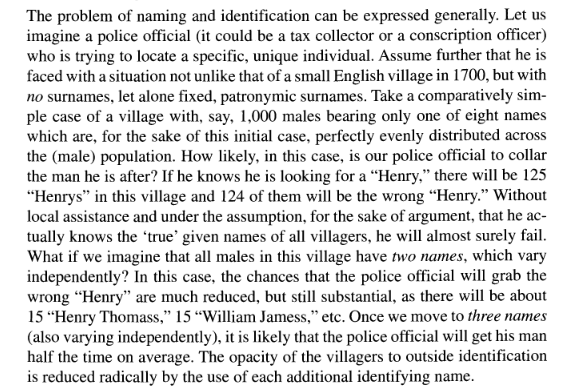
\includegraphics[scale=0.4]{subtex/scott9.png}
\end{frame}

\begin{frame}{California}

i

\end{frame}

\begin{frame}{China}


i

\end{frame}

\begin{frame}{Hawaii}

i

\end{frame}

\begin{frame}{Lithuania}

i

\end{frame}

\begin{frame}{Solutions and Strategies}

\begin{itemize}
\item Unicode
\item Passports
\item More
\end{itemize}

\end{frame}

\end{document}
